\documentclass[a4paper,11pt]{report}
\usepackage{chuan_math_gkt}
\usetikzlibrary{angles,quotes,intersections,patterns,decorations.pathreplacing}
\chuanexamsetup

\begin{document}
\examfontsize

\examsecret{绝密$\bigstar$启用前}

\examtitle{2022年普通高等学校招生全国统一考试（全国甲卷理科）}{数\quad 学}

\noticetitle
\begin{examnotice}
\item 答卷前，考生务必将自己的姓名、准考证号填写在答题卡上. 
\item 回答选择题时，选出每小题的答案后，用铅笔把答题卡上对应题目的答案标号涂黑. 如需改动，用橡皮擦干净后，再选涂其他答案标号. 回答非选择题时，将答案写在答题卡上. 写在本试卷上无效. 
\item 考试结束后，将本试卷和答题卡一并交回. 
\end{examnotice}

\examsection{一、选择题：本题共12小题，每小题5分，共60分. 在每小题给出的四个选项中，只有一项是符合题目要求的. }
\begin{examquestions}
\item 若 $z=-1+\sqrt3\mathrm{i}$，则 $\dfrac{z}{z\overline z-1}=$
\fourchoices{$-1+\sqrt3\mathrm{i}$}{$-1-\sqrt3\mathrm{i}$}{\tallchoice{$-\dfrac13+\dfrac{\sqrt3}{3}\mathrm{i}$}}{\tallchoice{$-\dfrac13-\dfrac{\sqrt3}{3}\mathrm{i}$}}

\item 某社区通过公益讲座以普及社区居民的垃圾分类知识. 为了解讲座效果，随机抽取10位社区居民，让他们在讲座前和讲座后各回答一份垃圾分类知识问卷，这10位社区居民在讲座前和讲座后问卷答题的正确率如下图：
\begin{tightcenter}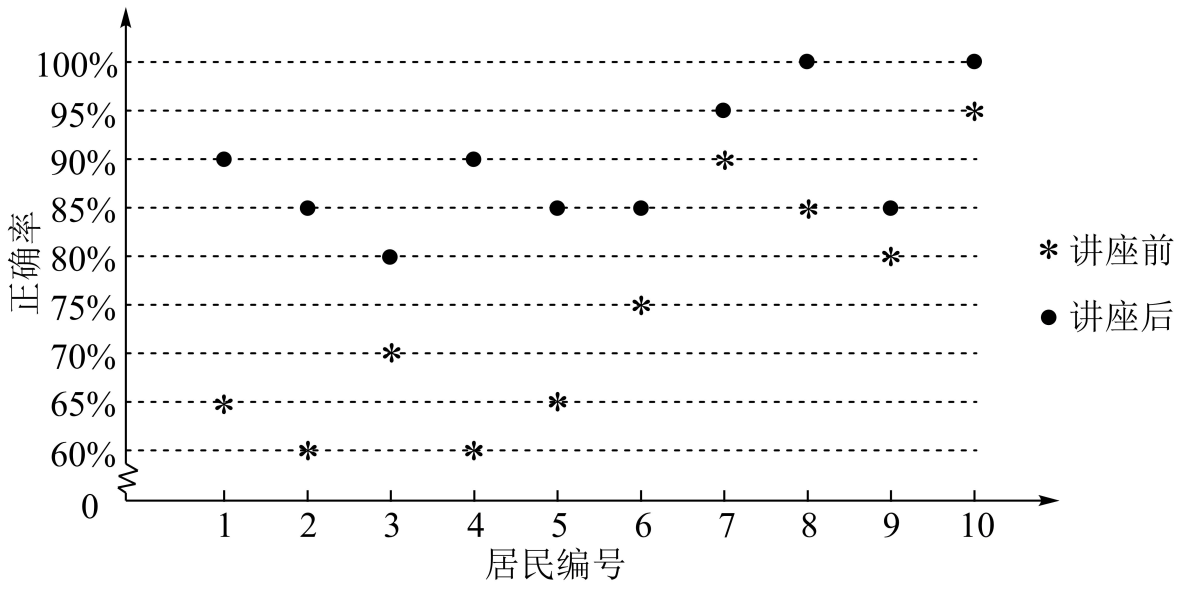
\includegraphics[width=10.5cm]{figures/2022_jiali_q2.png}\end{tightcenter}
则
\onechoices{讲座前问卷答题的正确率的中位数小于 $70\%$}{讲座后问卷答题的正确率的平均数大于 $85\%$}{讲座前问卷答题的正确率的标准差小于讲座后正确率的标准差}{讲座后问卷答题的正确率的极差大于讲座前正确率的极差}

\item 设全集 $U=\{-2,-1,0,1,2,3\}$，集合 $A=\{-1,2\}$，$B=\{x\mid x^2-4x+3=0\}$，则 $\complement_U(A\cup B)=$
\fourchoices{$\{1,3\}$}{$\{0,3\}$}{$\{-2,1\}$}{$\{-2,0\}$}

\item 如图，网格纸上绘制的是一个多面体的三视图，网格小正方形的边长为1，则该多面体的体积为
\begin{tightcenter}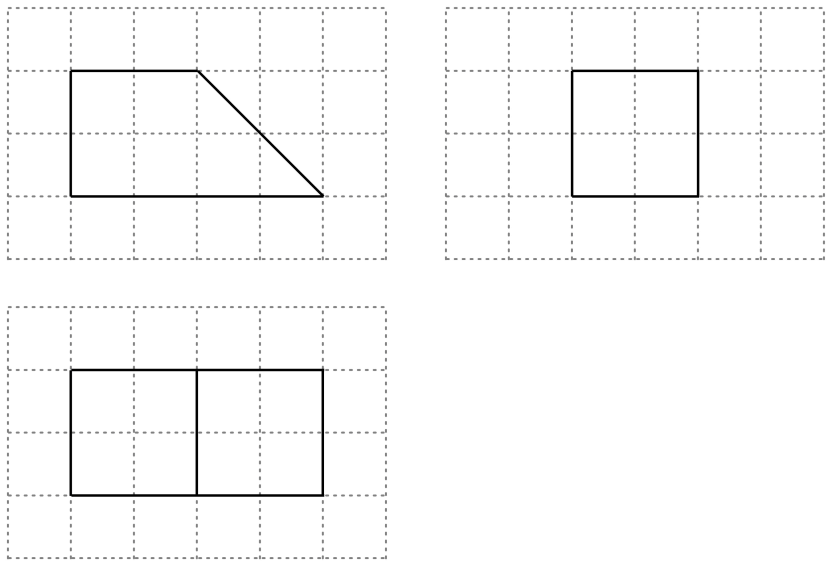
\includegraphics[width=6.8cm]{figures/2022_jiali_q4.png}\end{tightcenter}
\fourchoices{$8$}{$12$}{$16$}{$20$}

\item 函数 $y=(3^x-3^{-x})\cos x$ 在区间 $\left[-\dfrac\pi2,\dfrac\pi2\right]$ 的图象大致为
\graphchoices{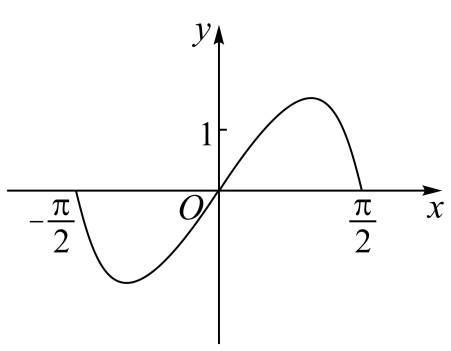
\includegraphics[width=4.3cm]{figures/2022_jiali_q5_A.png}}{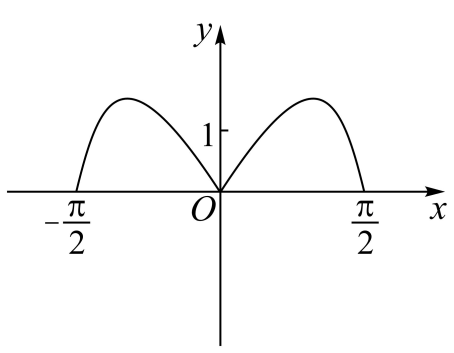
\includegraphics[width=4.3cm]{figures/2022_jiali_q5_B.png}}{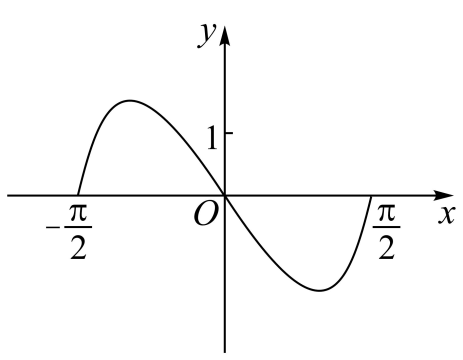
\includegraphics[width=4.3cm]{figures/2022_jiali_q5_C.png}}{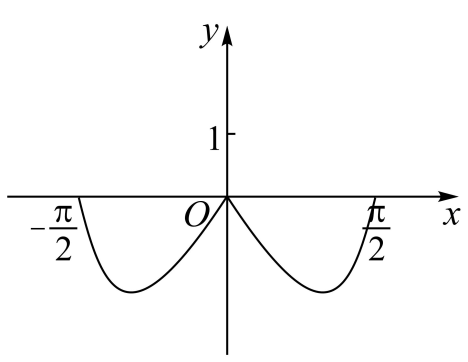
\includegraphics[width=4.3cm]{figures/2022_jiali_q5_D.png}}

\item 当 $x=1$ 时，函数 $f(x)=a\ln x+\dfrac bx$ 取得最大值 $-2$，则 $f'(2)=$
\fourchoices{$-1$}{\tallchoice{$-\dfrac12$}}{\tallchoice{$\dfrac12$}}{$1$}

\item 在长方体 $ABCD-A_1B_1C_1D_1$ 中，已知 $B_1D$ 与平面 $ABCD$ 和平面 $AA_1B_1B$ 所成的角均为 $30^\circ$，则
\twochoices{$AB=2AD$}{$AB$ 与平面 $AB_1C_1D$ 所成的角为 $30^\circ$}{$AC=CB_1$}{$B_1D$ 与平面 $BB_1C_1C$ 所成的角为 $45^\circ$}

\item 沈括的《梦溪笔谈》是中国古代科技史上的杰作，其中收录了计算圆弧长度的“会圆术”，如图，$\overset{\frown}{AB}$ 是以 $O$ 为圆心，$OA$ 为半径的圆弧，$C$ 是 $AB$ 的中点，$D$ 在 $\overset{\frown}{AB}$ 上，$CD\perp AB$. “会圆术”给出的 $\overset{\frown}{AB}$ 的弧长的近似值 $s$ 的计算公式：$s=AB+\dfrac{CD^2}{OA}$. 当 $OA=2,\angle AOB=60^\circ$ 时，$s=$
\begin{tightcenter}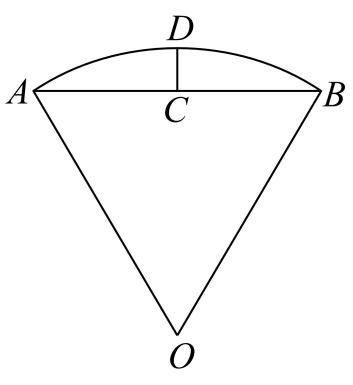
\includegraphics[width=4.0cm]{figures/2022_jiali_q8.png}\end{tightcenter}
\fourchoices{\tallchoice{$\dfrac{11-3\sqrt3}{2}$}}{\tallchoice{$\dfrac{11-4\sqrt3}{2}$}}{\tallchoice{$\dfrac{9-3\sqrt3}{2}$}}{\tallchoice{$\dfrac{9-4\sqrt3}{2}$}}

\item 甲、乙两个圆锥母线长相等，侧面展开图的圆心角之和为 $2\pi$，侧面积分别为 $S_\text{甲}$ 和 $S_\text{乙}$，体积分别为 $V_\text{甲}$ 和 $V_\text{乙}$. 若 $\dfrac{S_\text{甲}}{S_\text{乙}}=2$，则 $\dfrac{V_\text{甲}}{V_\text{乙}}=$
\fourchoices{$\sqrt5$}{$2\sqrt2$}{$\sqrt{10}$}{\tallchoice{$\dfrac{5\sqrt{10}}{4}$}}

\item 椭圆 $C:\dfrac{x^2}{a^2}+\dfrac{y^2}{b^2}=1(a>b>0)$ 的左顶点为 $A$，点 $P,Q$ 均在 $C$ 上，且关于 $y$ 轴对称. 若直线 $AP,AQ$ 的斜率之积为 $\dfrac14$，则 $C$ 的离心率为
\fourchoices{\tallchoice{$\dfrac{\sqrt3}{2}$}}{\tallchoice{$\dfrac{\sqrt2}{2}$}}{\tallchoice{$\dfrac12$}}{\tallchoice{$\dfrac13$}}

\item 设函数 $f(x)=\sin\left(\omega x+\dfrac\pi3\right)$ 在区间 $(0,\pi)$ 恰有三个极值点、两个零点，则 $\omega$ 的取值范围是
\fourchoices{\tallchoice{$\left[\dfrac53,\dfrac{13}{6}\right)$}}{\tallchoice{$\left[\dfrac53,\dfrac{19}{6}\right)$}}{\tallchoice{$\left(\dfrac{13}{6},\dfrac83\right]$}}{\tallchoice{$\left(\dfrac{13}{6},\dfrac{19}{6}\right]$}}

\item 已知 $a=\dfrac{31}{32}$，$b=\cos\dfrac14$，$c=4\sin\dfrac14$，则
\fourchoices{$c>b>a$}{$b>a>c$}{$a>b>c$}{$a>c>b$}
\end{examquestions}

\examsection{二、填空题：本题共4小题，每小题5分，共20分. }
\begin{examquestions}[start=13]
\item 设向量 $\vec a,\vec b$ 的夹角的余弦值为 $\dfrac13$，且 $|\vec a|=1$，$|\vec b|=3$，则 $(2\vec a+\vec b)\cdot\vec b=\blank$. 
\item 若双曲线 $y^2-\dfrac{x^2}{m^2}=1(m>0)$ 的渐近线与圆 $x^2+y^2-4y+3=0$ 相切，则 $m=\blank$. 
\item 从正方体的8个顶点中任选4个，则这4个点在同一个平面的概率为\blank. 
\item 已知 $\triangle ABC$ 中，点 $D$ 在边 $BC$ 上，$\angle ADB=120^\circ$，$AD=2$，$CD=2BD$. 当 $\dfrac{AC}{AB}$ 取得最小值时，$BD=\blank$. 
\end{examquestions}

\examsection{三、解答题：共70分. 解答应写出文字说明、证明过程或演算步骤. 第17题～第21题为必考题，每个试题考生都必须作答. 第22、23题为选考题，考生根据要求作答. }
\examsection{（一）必考题：共60分. }
\begin{examanswers}[start=17]
\item（12分）

记 $S_n$ 为数列 $\{a_n\}$ 的前 $n$ 项和. 已知 $\dfrac{2S_n}{n}+n=2a_n+1$. 

（1）证明：$\{a_n\}$ 是等差数列；

（2）若 $a_4,a_7,a_9$ 成等比数列，求 $S_n$ 的最小值. 

\item（12分）

在四棱锥 $P-ABCD$ 中，$PD\perp$ 底面 $ABCD$，$CD\parallel AB$，$AD=DC=CB=1$，$AB=2$，$DP=\sqrt3$. 

\noindent\begin{minipage}[t]{0.62\linewidth}
（1）证明：$BD\perp PA$；

（2）求 $PD$ 与平面 $PAB$ 所成的角的正弦值. 
\end{minipage}\hfill
\begin{minipage}[t]{0.32\linewidth}
\vspace{-1.4em}\centering
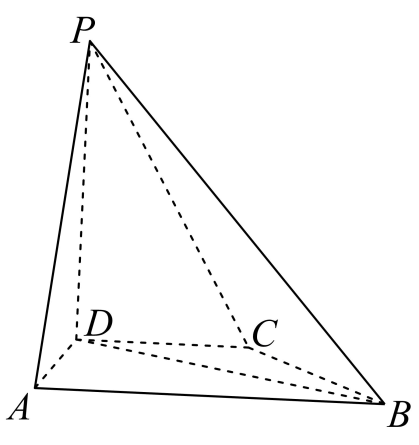
\includegraphics[width=\linewidth]{figures/2022_jiali_q18.png}
\end{minipage}

\item（12分）

甲、乙两个学校进行体育比赛，比赛共设三个项目，每个项目胜方得10分，负方得0分，没有平局. 三个项目比赛结束后，总得分高的学校获得冠军. 已知甲学校在三个项目中获胜的概率分别为0.5，0.4，0.8，各项目的比赛结果相互独立. 

（1）求甲学校获得冠军的概率；

（2）用 $X$ 表示乙学校的总得分，求 $X$ 的分布列与期望. 

\item（12分）

设抛物线 $C:y^2=2px(p>0)$ 的焦点为 $F$，点 $D(p,0)$，过 $F$ 的直线交 $C$ 于 $M,N$ 两点. 当直线 $MD$ 垂直于 $x$ 轴时，$|MF|=3$. 

（1）求 $C$ 的方程；

（2）设直线 $MD,ND$ 与 $C$ 的另一个交点分别为 $A,B$，记直线 $MN,AB$ 的倾斜角分别为 $\alpha,\beta$. 当 $\alpha-\beta$ 取得最大值时，求直线 $AB$ 的方程. 

\item（12分）

已知函数 $f(x)=\dfrac{e^x}{x}-\ln x+x-a$. 

（1）若 $f(x)\geq0$，求 $a$ 的取值范围；

（2）证明：若 $f(x)$ 有两个零点 $x_1,x_2$，则 $x_1x_2<1$. 
\end{examanswers}

\examsection{（二）选考题：共10分. 请考生在第22、23题中任选一题作答. 如果多做，则按所做的第一题计分. }
\begin{examanswers}[start=22]
\item（10分）【选修4-4：坐标系与参数方程】

在直角坐标系 $xOy$ 中，曲线 $C_1$ 的参数方程为\linsys{x=\dfrac{2+t}{6},\\ y=\sqrt t}（$t$ 为参数），曲线 $C_2$ 的参数方程为\linsys{x=-\dfrac{2+s}{6},\\ y=-\sqrt s}（$s$ 为参数）. 

（1）写出 $C_1$ 的普通方程；

（2）以坐标原点为极点，$x$ 轴正半轴为极轴建立极坐标系，曲线 $C_3$ 的极坐标方程为 $2\cos\theta-\sin\theta=0$，求 $C_3$ 与 $C_1$ 交点的直角坐标，及 $C_3$ 与 $C_2$ 交点的直角坐标. 

\item（10分）【选修4-5：不等式选讲】

已知 $a,b,c$ 均为正数，且 $a^2+b^2+4c^2=3$，证明：

（1）$a+b+2c\leq3$；

（2）若 $b=2c$，则 $\dfrac1a+\dfrac1c\geq3$. 
\end{examanswers}

\end{document}
